\documentclass{report}
\usepackage[utf8]{inputenc}
\usepackage{amsmath}
\usepackage{amsfonts}
\usepackage{listings}
\usepackage{graphicx}
\usepackage[table]{xcolor}
\usepackage{caption}
\usepackage{url}
\usepackage{fancyhdr}


\pagestyle{fancy}
\fancyhead{}
\fancyhead[L]{Johan Wikström - Anaël Bonneton}
\fancyfoot{}

\begin{document}
\title{Modeling the zombie apocalypse using a HIZD-model and HPC}
\author{Johan Wikström - 645714 \\
        Anaël Bonneton - 646275}
\maketitle
\tableofcontents

\newpage

\section{Problem description}	

\paragraph{}
SIR-models (Susceptible, Infected, Removed/Recovered) are commonly used to model diseases in populations. In this report, we use a modified SIR-model called a HIZD-model (Human,Infected, Zombie, Decayed) to model a potential zombie apocalypse. The aim of the report is to determine the effect of some vital parameters, such as the infection risk when encountering a zombie, the incubation time for an infected human, on the survival of the human and zombie populations. In order to speed up the computation, we have used multi-threading and MPI\cite{openmpi}. We have run the simulation on an IBM iDataplex x86 system with up to 256 MPI processes at once. In the interest of animal protection, we aim to get a model where the zombies and humans both have stable populations.

\section{Model}

\paragraph{}
The simulation takes place in a fictional continent about the size of Australia, 8000000 km\textsuperscript{2}. In order to model this geographical area we use 128 250x250 meshes where each square represents 1 km\textsuperscript{2}. Each square can be inhabited or empty. There are three types of inhabitants : \emph{humans}, \emph{infected} and \emph{zombies}. This is a sparsely populated area as is the case in most sources regarding the zombie apocalypse\cite{zombieland}. In our model, the time granularity is days.

In our model we have a number of variable factors, some relatively known and some unknown that can be changed to model different outcomes of the zombie apocalypse.

\begin{itemize}
\item \emph{Human death rate}: The average human death rate per person, per day
\item \emph{Human birth rate}: The average birth rate per human per day
\item \emph{Brain eating probability}: The probability that a human is infected by a zombie of the collide, i.e. occupy the same square.
\item \emph{Infected to zombie probability}: The probability that an infected human will turn into a zombie on any given day.
\item \emph{Human move probability}: The probability that a human will move outside of a 1x1 km\textsuperscript{2} radius on any given day.
\item \emph{Zombie move probability}: The probability that a zombie will move outside of a 1x1 km\textsuperscript{2} radius on any given day.
\end{itemize}

\subsection{Humans}
\paragraph{}
The initial population statistics of our humans were based on actual Australian population data (table~\ref{AustralianData}), but in this simulation we assume a very sparsely populated land mass which is more coherent with our sources on the matter\cite{zombieland} . The humans in our model move in random directions, much like real humans do in a crisis, and this assumption has also been made in earlier works\cite{munz}. Humans can only move at a maximum pace of one square kilometer per day and they can only move in the directions up, down, left and right. When a human moves into a square inhabited by a zombie there is a probability that the human gets bitten and turns into a zombie. The probability of infection when in the same area as a zombie is currently unknown and in the model, we experiment with different values for this probability. In case of a zombie apocalypse, the authors recommend determining this parameter through empirical studies, placing a human and a zombie in the same square kilometer, measuring the time to infection to estimate the brain eating probability.
\begin{table}[!h]
\centering
    \begin{tabular}{|l|l|}
      \hline
        Birth rate & 13.3 per year per 1000 persons \\
      \hline
        Death rate & 6.5 per year per 1000 persons \\
      \hline
\end{tabular}
\caption{Northern Territory demographic data}\label{AustralianData}
\end{table}

\paragraph{}
Most of the humans' daily moving are within a kilometer. In our simulation, the probability for a human to travel more than 1 kilometer in one day is 0.4. When a human encounters a zombie, it may become infected with the probability of 0.65.

\subsection{Zombies}
The life of the zombie is largely unknown. We do not know how fast they move, how long before they decompose or how long the zombie incubation time is. For this reason, several parameters in our model can be adjusted to fit different apocalyptic scenarios. One thing that we discovered is that in a sparsely populated land, if we started with just two zombies, the probabilities of these zombies to infect any body before they decomposed was quite low. Therefore, to get reasonable data we started with an extremely small zombie population of around 250 zombies to more easily run the simulations.

\subsection{Infected humans}
The incubation time of the zombie virus is also largely unknown so this parameter is variable in our model. During the incubation period an infected cannot infect other humans. However, the power of the zombie virus during the incubation time is so powerful that infected humans cannot die like humans, or decompose like zombies. Judging by our sources\cite{deadheads}, a person bitten by a zombie gets a radically lowered risk of dying, almost always surviving until the point of zombiefication. After that, point however, the risk of dying by headshot is radically increased.

\subsection{Parallelisation of the model}
\subsubsection{MPI}
<<<<<<< HEAD
The model is divided into several small meshes that are on the order of 60000 cells big. Each of these small meshes are connected to four neighbors and the universe wraps around. Before each timestep, the outer cells of each mesh are exchanged with the neighboring meshes which allows for inhabitants to move between meshes. This can create collisions if two inhabitants from two different meshes move into the same cell but this is mostly resolved with a very simple mechanism. If a collision is detected, two other nearby cells are examined and if any of these is empty, one of the colliding parties are moved. This may still lead to collisions if the populations density is very high but in a small experiment, this simple solution reduced collisions with over 99\% which was deemed enough for this application, as shown in Tab.~\ref{collisions}.
=======
\paragraph{}
The model is divided into several small meshes that are on the order of 60000 cells big. Each of these small meshes are connected to four neighbours and the universe wraps around. Before each timestep, the outer cells of each mesh are exchanged with the neighbouring meshes which allows for inhabitants to move between meshes. This can create collisions if two inhabitants from two different meshes move into the same cell but this is mostly resolved with a very simple mechanism. If a collision is detected, two other nearby cells are examined and if any of these is empty, one of the colliding parties are moved. This may still lead to collisions if the populations density is very high but in a small experiment, this simple solution reduced collisions with over 99\% which was deemed enough for this application (table~\ref{collisions}).
>>>>>>> 0b7230c7a02995e7fbf5c178fe6eb243fa4815df

\begin{table}[h!]
\centering
\begin{tabular}{|l|l|}
\hline
& Collisions\\
\hline
Before & 675\\
\hline
After & 6\\
\hline
\end{tabular}
\caption{The number of collisions per 1000 timesteps on four 98x98 grids before and after collision handling}
\label{collisions}
\end{table}

\subsubsection{Multi-threading}

\paragraph{}
In order to do the computation on each small mesh we use multi-threading. Each thread do the computation for some columns of the mesh. As the computation requires the closest neighbours, when a thread works on the column $j$, the columns $j-1$ and $j+1$ cannot be used by other threads. In order to make sure there is no confict, we use \emph{locking}.

\paragraph{}
We had to deal with another confilt during the computation of the statistics. In order to save time, we update the statistics after each event (birth, death, getting infected, etc $\cdots$), instead of computing the statistics at the end of each iteration. However, with this method, two threads may update the statistics at the same time. In order to avoid this kind of conflict, a first solution was locking. However, there are so many events which require to upadte the statistics, that the locking is really too time consuming when the number of threads increase. The second solution, the one we are using, is each thread computes its local statistics and at the end of each iteration the main thread computes the global statistics thanks to the local ones.



\section{Results}
%% TODO graphs !!!!!!!!!!!!!

%%% compare the evolution of the humans with and without the zombies
%%%     compare the population growth

Without the zombies, the human population growth is slow and steady, about 1\% per year as seen in Fig.~\ref{withoutzombies}. But with zombies, the population dynamics vary considerably as can be seen in Fig.~\ref{stable}. One thing we noticed very early was that it is not easy to achieve a world where zombies and humans could coexist. If we made the zombies too ferocious (increased their movement, decreased their decomposition rate and increased the brain eating probability) they quickly wiped out much of the human population but were the wiped out themselves since there were not enough humans left to sustain a zombie population. This is shown in Fig.~\ref{zombieswipedout}.

\begin{figure}
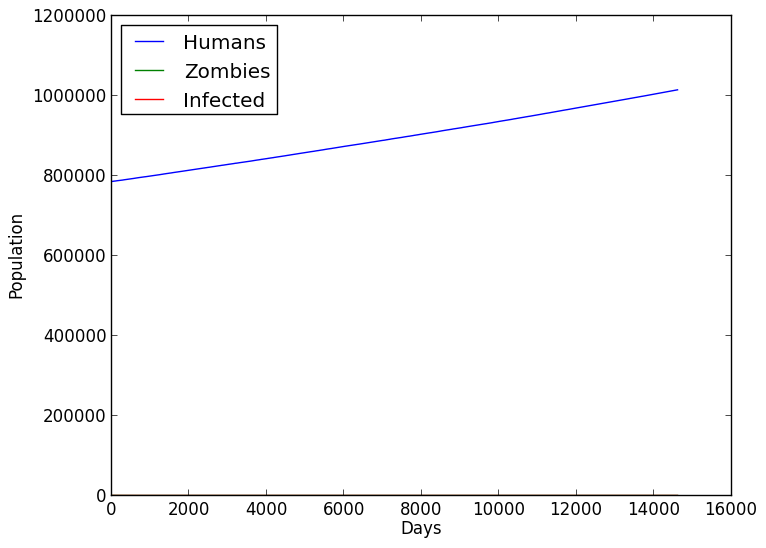
\includegraphics[width=350pt]{plots/withoutzombies}
\caption{A graph over the the human population in a world without zombies.}
\label{withoutzombies}
\end{figure}
\begin{figure}
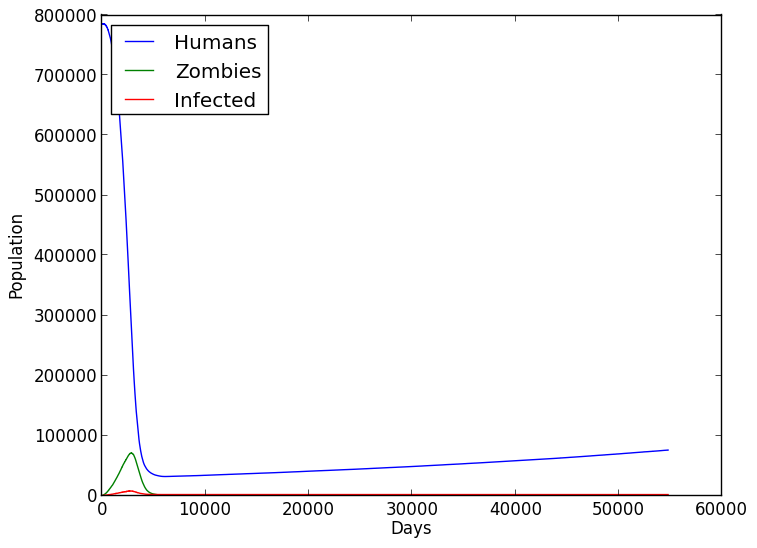
\includegraphics[width=350pt]{plots/zombieswipedout}
\caption{An example of when the zombie population brings it's own downfall. In this 150 year simulation the brain eating probability is high(0.5) and the zombie decomposition risk is low(0.005) but the zombies are quickly wiped out due to lack of food.}
\label{zombieswipedout}
\end{figure}



%%% over the years, evolution of nb of humans, nb of zombies and infected
%%% per year (average) : number of infected

\section{Discussion of results}
\begin{thebibliography}{99}
\bibitem{openmpi}
Open MPI: Goals, Concept, and Design of a Next Generation MPI Implementation. Edgar Gabriel, Graham E. Fagg, George Bosilca, Thara Angskun, Jack J. Dongarra, Jeffrey M. Squyres, Vishal Sahay, Prabhanjan Kambadur, Brian Barrett, Andrew Lumsdaine, Ralph H. Castain, David J. Daniel, Richard L. Graham, and Timothy S. Woodall. In Proceedings, 11th European PVM/MPI Users' Group Meeting, Budapest, Hungary, September 2004
\bibitem{munz}
Munz, Philip, et al. "When zombies attack!: mathematical modelling of an outbreak of zombie infection." Infectious Disease Modelling Research Progress 4 (2009): 133-150.
\bibitem{deadheads}
Brett Pierce, Drew T. Pirece(writers,directors), 2011, Deadheads
\bibitem{zombieland}
Fleischer, R., Reese R., Wernick P., 2009, Zombieland 
\end{thebibliography}
\end{document}
